\section{Implementation}

% serial vs. parallel approaches
Hash tables can be implemented with a myriad of different techniques,
but are traditionally implemented sequentially as an array of pointers to
objects. Parallel implementations typically distribute table data
across nodes, requiring that the hash table stores the entire object
and not simply a reference. 

\subsection{PDHT Programming Model}


% parallel programming model
%  - key/value pairs
%  - object can be located anywhere distributed memory, governed
%     solely by hash function
%  - hash function maps key -> rank/offset tuple
%  - two primary operations put/get
%     - if put yields a collision, then object is placed in next
%        available bucket
%     - get returns object, probing as necessary
 
The PDHT system provides a distributed key/value store within a
high-performance computing cluster. A hash function maps the object
key to a rank and offset tuple, identifying each distinct location
within the hash table. PDHT provides the two primary {\em put} and
{\em get} operations to store and fetch items from the table. Since
multiple keys may hash to the same table location (a collision), PDHT
implements a linear probing behavior. If a {\em put} yields a
collision, the object is then placed in the next available bucket on
the same processor rank. The {\em get} operation also checks for
collisions and searches accordingly. 

% considerations:
%  - two-sided communication not amenable to hash table implementation
%  - one-sided will rely on MPI-2+, UPC, or some other PGAS-ish
%     approach
Two-sided communication is not inherently amenable to implementing a
high-performance hash table. Hash tables rely on fine-grained, random
data access which makes a message-passing based implementation
challenging. Several existing approaches have been built upon
one-sided models using MPI-2, UPC, and other PGAS approaches.

\subsection{Portals 4}
% portals background
%  define NI, PTE
%  define matching, ME, matching lookup process
%  define counters and events

A primary motivation for using a one-sided approach is to allow
RDMA-based memory accesses to fetch remote data without interupting
the processor core on the far end. We can take advantage of NIC
hardware offload to a greater extent than conventional PGAS approaches
by using low-level communication primitives provided by the Portals 4
network interface specification. Portals defines a number of
abstractions and concepts that are necessary to understanding the PDHT
implementation.

Portals specifies a {\em network interface} (NI) as a per-process
abstraction of a physical network interface. Each NI is associated
with a portal table. The index into the portal table is specified on
every Portals communication operation and is used to separate and
classify different channels between endpoints.

Each portal table entry (PTE) maintains a list of memory regions that are
available for communication operations as well as an event queue to
track asynchronous notifications for ongoing communication. Portals
provides two distinct lists: {\em matching lists} that support
two-sided message passing systems and {\em non-matching lists} that
support one-sided communication models. PDHT relies on the matching
features of Portals and will be the focus of the remainder of the
implementation discussion.

A PTE using the matching interface maintains a list of match-list
entries (ME). Each ME specifies a set of matching criteria and a
memory region associated with the entry. If all of the match criteria
are satisfied, the communication operation commences working on
corresponding memory region. In particular, each ME contains a 64-bit
{\em match bits} field that must match exactly for an incoming
communication to proceed with the given ME. For example, a process
would post an {\tt MPI\_Recv()} with a specific match bits
field. Later, Portals would receive a communication request for an
{\tt MPI\_Send()} with the same match bits, which would be correspond
to the posted receive.

Additionally, Portals provides both {\em event queues} and {\em event
  counters} to track the data movement in and out of memory regions
used by Portals operations. Both events and counters are also used to
log failure events and other information.


\subsection{PDHT Implementation}

% use figure* to span both cols
\begin{figure}[ht]
  \centering
  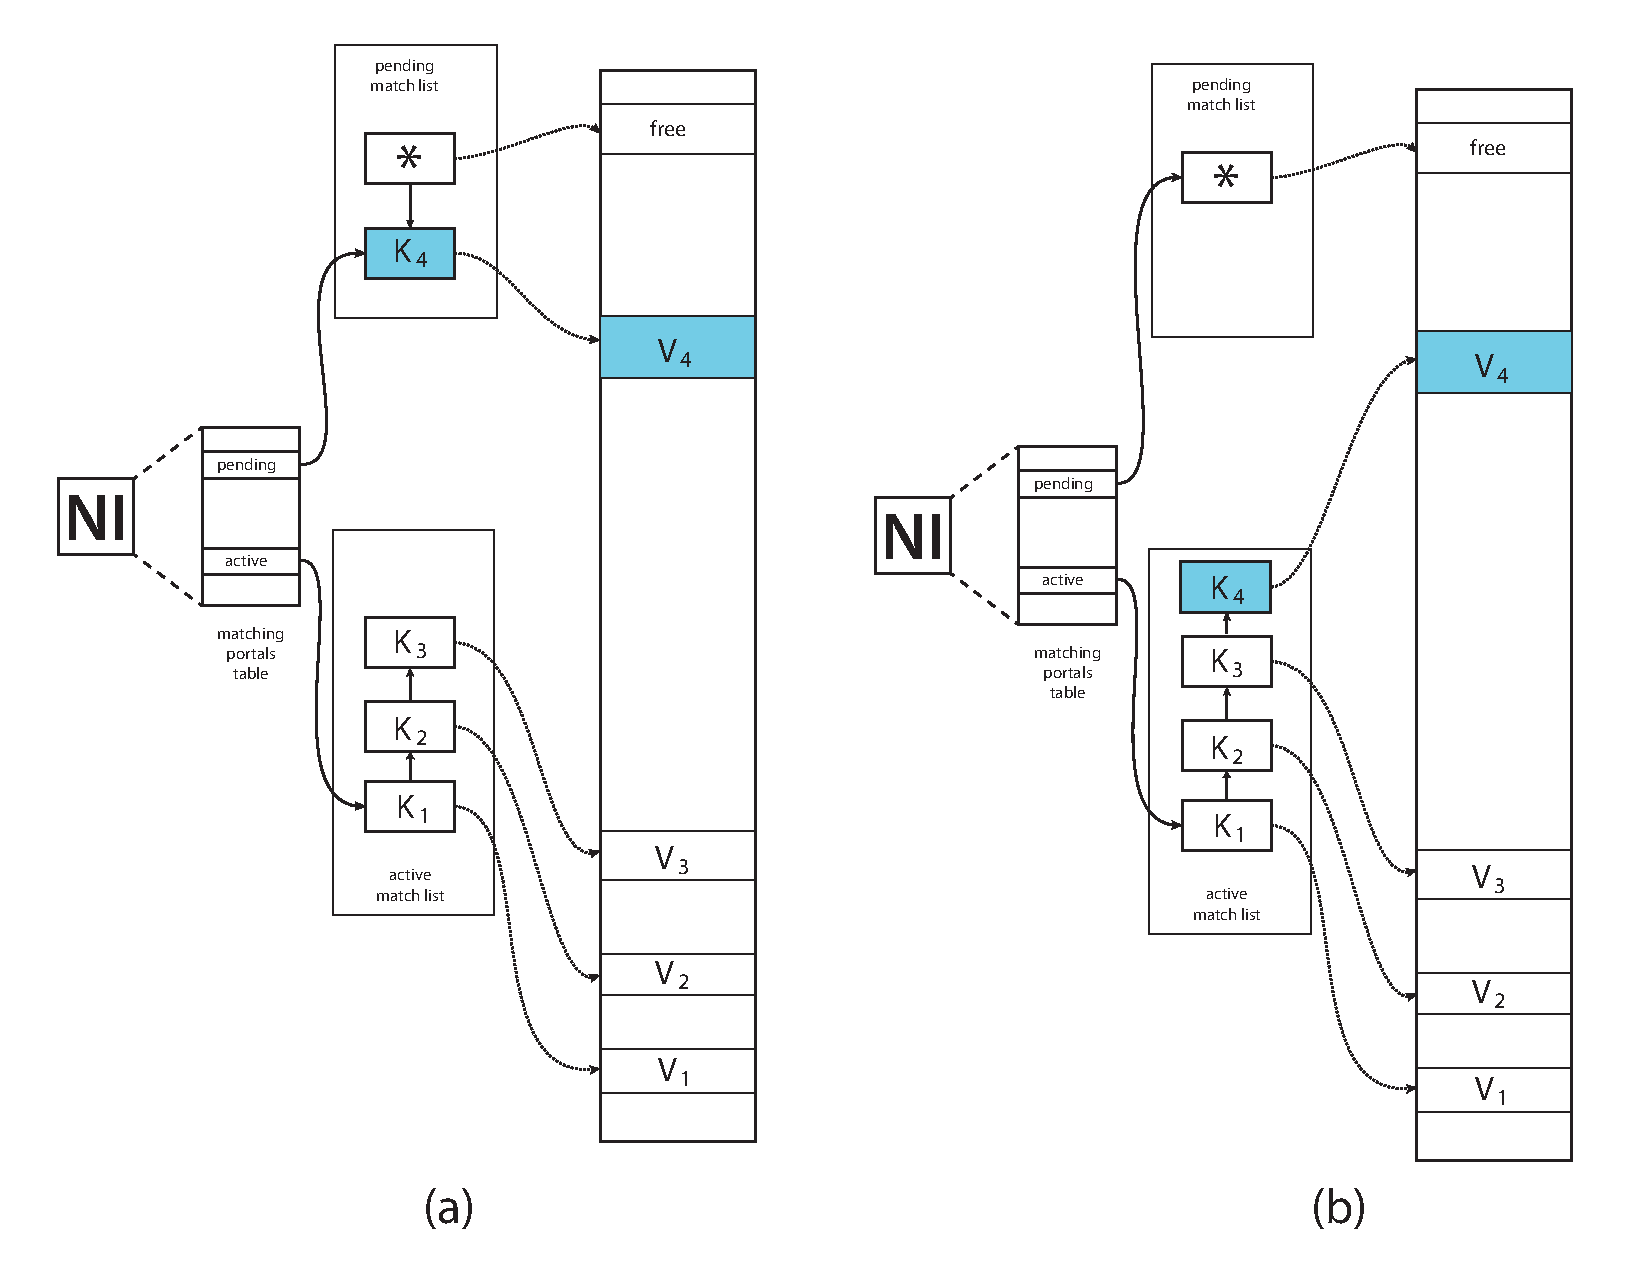
\includegraphics[width=3in]{figs/put_smaller}
  \caption{Slow motion {\tt put()} operation}
  \label{fig:put}
\end{figure}

\begin{figure}[ht]
  \centering
  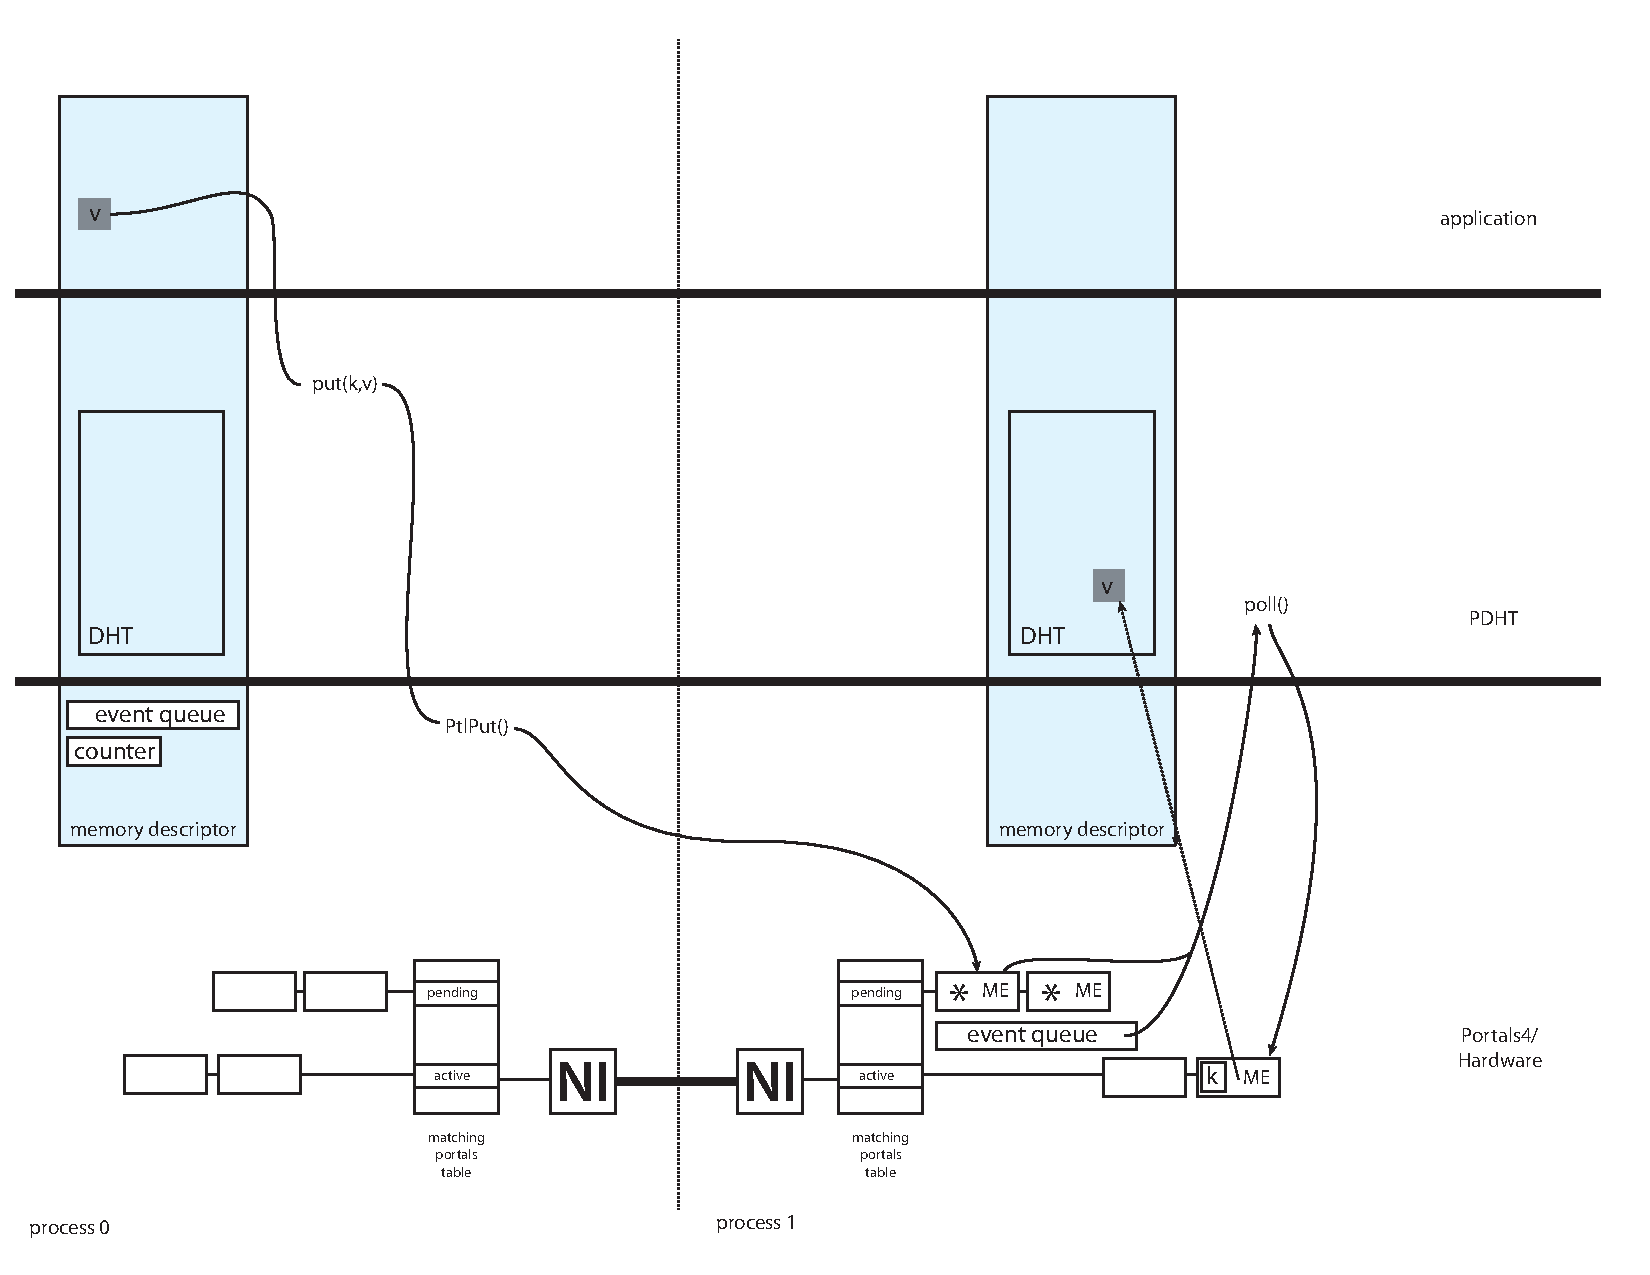
\includegraphics[width=3in]{figs/hwsw}
  \caption{Hardware/Software Abstractions}
  \label{fig:hwsw}
\end{figure}

% implementation
%  - array of objects + metadata
%  - pending ME list 
PDHT supports multiple hash tables per-process. Each hash table is
treated as a distributed array of value objects and a small amount of
metadata per entry. Upon initialization, PDHT opens a Portals NI with
two distinct portal table entries, one for {\em pending} match list
entries and another for {\em active} match list entries. The pending
match list is filled with a number of entries that will match any
incoming communication request. Each match list entry corresponds to a
local memory region that can contain a single entry in the hash table
array structure.

The key idea within PDHT is to create a match list entry (ME) for each
active element in the hash table. The hash function maps the key to a
64-bit value used as the match bits field for the Portals
communication request. By relying on the matching interface to handle
hash entries, much of the servicing of a get request can be relegated
to Portals, which in turn rely on hardware acceleration.

% put operation
%  - run hash to determine rank/offset
%  - figure 1
%  - active ME list
%  - migration from pending to active

To insert a new element into the hash table, the process first hashes
the key, giving both the target processor rank and the 64-bit match
bits field used for the value. Next, the process performs a one-sided
put operation on the pending PTE, using one of the wildcard entries on
the match list. The hash table value data is communicated and stored
into the memory region defined by the match list entry. As can be seen
in Figure \ref{fig:put}a, the table entry data resides on the owner
process, but the match-list entry is still resident on the pending
PTE, rather than the active one. To complete the put operation, the
used up entry on the pending PTE needs to be replaced with a new empty,
wildcard ME and the new hash table object needs to have an entry on
the active PTE, with the match bits set to correspond to the hashed
key. This state can be seen in Figure \ref{fig:put}b. 

% - polling approach
The most straightforward approach to moving the ME from the pending
match list to the active list is by relying on a progress
thread. Portals provides blocking wait and polling routines to check
for new event notifications or counter changes. When a process
receives a put operation and updates the pending match list, a Portals
event is generated and appended to the event queue. When the progress
thread sees this event, it creates a replacement wildcard entry for
the pending queue that references an empty element in the hash table
array. It also creates a new ME with the appropriate match bits and
appends it to the active list. Any subsequent get requests will be
able to find a match in the active PTE.


% - triggered append approach


% get operation
%  - run hash
%  - issue PtlGet from active list
%  - check for collision


%  - custom hash functions 
%  - 64-bit hash space, rather than array bucket
%      - detach key -> array size dependency
%      - lower collision rates

% other operations
%  - iteration
%  - non-blocking / bundled puts/gets
%  - interoperability


%%% Local Variables: 
%%% mode: latex
%%% TeX-master: "paper"
%%% End: 
